\section{Linear IC}

\subsection{Pengantar}
\begin{frame}{Linear IC}
	\begin{itemize}
		\item Op amp : $\frac{1}{3}$ bagian dari IC
		\item Linear IC : op amp, audio amplifier, video amplifier, voltage regulator
	\end{itemize}
\end{frame}

\subsection{Tabel Op Amp}
\begin{frame}{Tabel Parameter Op Amp saat 25$^{\circ}$}
	\begin{center}
		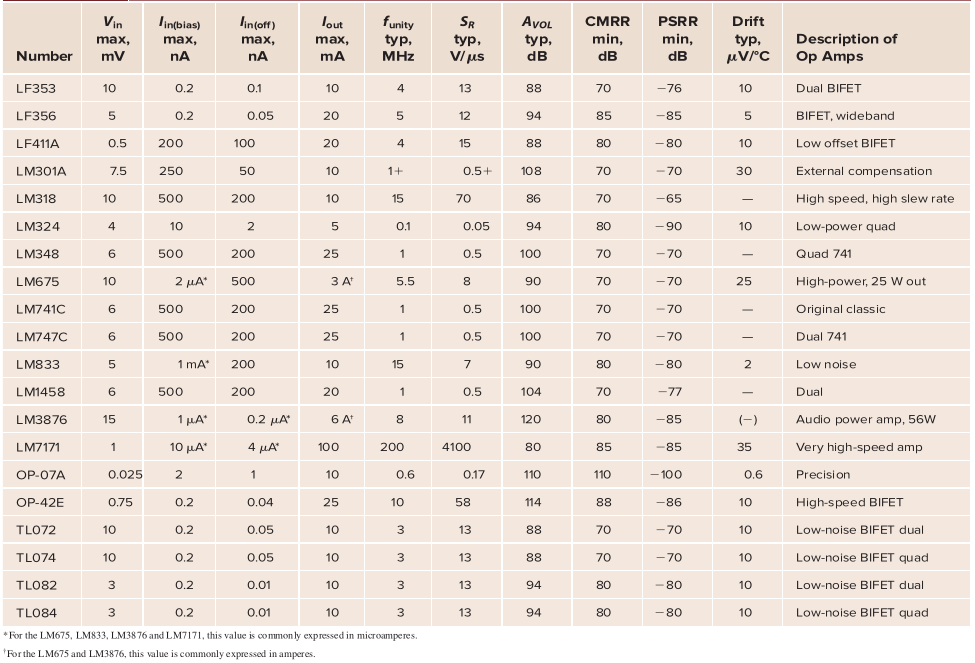
\includegraphics[height=0.8\textheight]{gambar/table-16.3}
	\end{center}
\end{frame}

\begin{frame}{Power Supply Rejection Ration (PSRR)}
	\begin{itemize}
		\item Persamaan PSRR:
			\begin{equation}\label{pers.16.17}
				PSRR = \frac{\Delta V_{in(off)}}{\Delta V_S}
			\end{equation}
		\item PSRR dari LF353 = -76 dB $ \rightarrow $ PSRR = $ 10^(-76/20) = 0.000158 = 158 ~\mu\text{V}/\text{V}$
		\item Setiap perubahan pada tegangan supply sebesar 1 V akan menyebabkan perubahan tegangan offset input sebesar 158 $ \mu $V
	\end{itemize}
\end{frame}

\begin{frame}{Drift}
	\begin{itemize}
		\item Koefisien temperatur dari tegangan offset input
		\item Seberapa banyak tegangan offset input akan meningkat karena temperatur
		\item Drift dari LF353 = 10 $ \mu $V/$ ^{\circ} $C $ \rightarrow $ tegangan offset input akan meningkat sebesar 10 $ \mu $V untuk setiap kenaikan 1 $ ^\circ $C
		\item Jika temperatur internal dari op amp meningkat sebesar 50 $ ^{\circ} $C maka tegangan offset input dari LF353 meningkat sebesar 500 $\mu$V
	\end{itemize}
\end{frame}

\subsection{Audio Amplifiers}
\begin{frame}{Audio Amplifiers}
	\begin{itemize}
		\item Preamps = audio amplifier dengan daya output $ < $ 50 mW
		\item Front-end audio system
		\item Mengurangi low noise dari optical sensors, magnetic tape heads, microphones, dll
		\item Contoh:
		\begin{itemize}
			\item LM833: low-noise dual preamp, $ A_v =$ 110 dB, 27-V power bandwidth 120 kHz, input berupa diff amp
		\end{itemize}
	\end{itemize}
\end{frame}

\begin{frame}{Audio Amplifiers}
	\begin{itemize}
		\item Medium-level audio amplifiers = output power 50 mW - 500 mW
		\item Near output end
		\item Portable electonic devices: cell phones, CD player
		\item Contoh:
		\begin{itemize}
			\item LM4818 audio power amplifier: output power 350 mW
		\end{itemize}
	\end{itemize}
\end{frame}

\begin{frame}{Audio Amplifiers}
	\begin{itemize}
		\item Output power $ > $ 500 mW
		\item High-fidelity amplifier, intercoms, AM-FM radio
		\item Contoh:
		\begin{itemize}
			\item LM380: $ A_v = $ 34 dB, bandwidth 100 kHz, output power 2 W
			\item LM4756: $ A_v = $ 30 dB, output power 7 W/channel
		\end{itemize}
	\end{itemize}
\end{frame}

\subsection{Video Amplifiers}
\begin{frame}{Video Amplifiers}
	\begin{itemize}
		\item Wideband amplifier
		\item Flat response (constant decibel voltage gain)
		\item Very broad range of frequencies
		\item Applications in which the range of input frequencies is very large: analog oscilloscopes, video cameras, copiers and scanners, and HDTV amplifiers
		\item Contoh:
		\begin{itemize}
			\item LM7171: very high-speed amplifier, wide unity-gain bandwidth of 200 MHz, slew rate of 4100 V/$ \mu $S
			\item NE592: voltage gain 52 dB, cutoff frequency 40 MHz, voltage gains and bandwidths dapat diatur dengan menghubungkan external resistors yang berbeda sehingga menjadi 90 MHz
			\item MC1553: gain 52 dB, bandwidth 20 MHz, adjusted by changing
			external components
			\item LM733: up to 20-dB gain, bandwidth of 120 MHz (adjusted by changing external components)
		\end{itemize}
	\end{itemize}
\end{frame}

\subsection{Voltage Regulator}
\begin{frame}{Voltage Regulator}
	\begin{itemize}
		\item Rectifier $ \rightarrow $ dc voltage + ripple $ \rightarrow $ voltage regulator
		\item DC voltage $ \propto $ line voltage
		\item Perubahan 10\% dari line voltage $ \propto $ perubahan 10\% DC voltage $ \leftarrow $ ini terlalu besar
		\item LM340 series $ \rightarrow $ menahan perubahan 0.01\%, positive/negative output, adjustable output voltage, and short-circuit protection.
	\end{itemize}
\end{frame}